\chapter{Bitwise Operations and XOR}
\chapterepigraph{Bits are independent until a carry says otherwise. Almost
every bitwise problem is solved by one of two moves: look at each bit
separately, or build the answer from the highest bit down.}

\section{Theory and Must-Know Patterns}
\label{sec:bit-theory}

\subsection*{The operators}

\begin{center}
\renewcommand{\arraystretch}{1.2}
\begin{tabular}{cccccc}
\toprule
$x$ & $y$ & $x\,\&\,y$ & $x\mid y$ & $x\oplus y$ & C++ \\
\midrule
0&0&0&0&0& \texttt{\&}, \texttt{|}, \texttt{\^{}}\\
0&1&0&1&1& \texttt{x << k} $=x\cdot2^k$\\
1&0&0&1&1& \texttt{x >> k} $=\lfloor x/2^k\rfloor$\\
1&1&1&1&0& \texttt{\_\_builtin\_popcountll(x)}\\
\bottomrule
\end{tabular}
\end{center}

\subsection*{Identities you will use every contest}

\begin{itemize}
  \item $x\oplus x=0$, $x\oplus0=x$, $\oplus$ is associative and commutative:
        \textbf{xor is its own inverse}. Hence $a\oplus c=b\iff c=a\oplus b$.
  \item $x+y=(x\oplus y)+2(x\,\&\,y)$. Therefore $x\oplus y\le x+y$ with
        equality iff $x\,\&\,y=0$ (no carries).
  \item $x\,\&\,(x-1)$ clears the lowest set bit; $x\,\&\,(-x)$ isolates it.
  \item Bit $b$ of $x$: \texttt{(x >> b) \& 1}. Highest set bit:
        $63-\texttt{\_\_builtin\_clzll}(x)$.
  \item \textbf{Prefix xor:} with $P_0=0$, $P_i=a_1\oplus\dots\oplus a_i$, the
        xor of $a_\ell..a_r$ is $P_r\oplus P_{\ell-1}$.
  \item $0\oplus1\oplus\dots\oplus(2^M-1)=0$ for $M\ge2$.
  \item A number $v$ has at most $2^{\text{popcount}(v)}$ submasks; iterate
        them with \texttt{for (s = v; s; s = (s - 1) \& v)}.
\end{itemize}

\subsection*{Pattern 1: bits are independent}

AND, OR and XOR act on each bit separately. If a condition is a combination
of these operations, decide it \emph{bit by bit} (Bitwise Reversion,
Tatar-style parity arguments). Addition breaks independence through carries
--- that is when you need a digit DP over bits (Jackpot).

\subsection*{Pattern 2: greedy from the highest bit}

Bit $b$ is worth more than all lower bits together ($2^b>2^b-1$). So to
maximise a value, fix bits from the top: take bit $b$ whenever some completion
still exists (largest submask $\le x$, maximum xor pair in a trie).

\subsection*{Pattern 3: xor linear algebra}

Treat numbers as vectors over $\mathbb{F}_2$. A \textbf{xor basis} (Gaussian
elimination on bits) answers ``can $v$ be written as a xor of a subset?'' in
$O(\log V)$ and has at most $\lceil\log_2 V\rceil$ elements.

\begin{center}
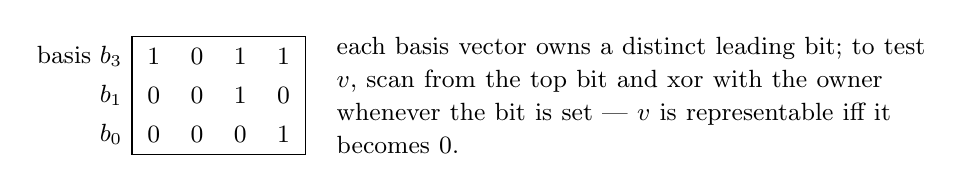
\begin{tikzpicture}[x=0.55cm,y=0.5cm]
  \node[left] at (0,2) {\small basis $b_3$}; \node[left] at (0,1) {\small $b_1$};
  \node[left] at (0,0) {\small $b_0$};
  \foreach \i/\v in {0/1,1/0,2/1,3/1} {\node at (\i+0.5,2) {\small \v};}
  \foreach \i/\v in {0/0,1/0,2/1,3/0} {\node at (\i+0.5,1) {\small \v};}
  \foreach \i/\v in {0/0,1/0,2/0,3/1} {\node at (\i+0.5,0) {\small \v};}
  \draw (0,-0.5) rectangle (4,2.5);
  \node[right,text width=7.5cm,align=left] at (4.5,1) {\small each basis vector owns a distinct
  leading bit; to test $v$, scan from the top bit and xor with the owner
  whenever the bit is set --- $v$ is representable iff it becomes $0$.};
\end{tikzpicture}
\end{center}

\subsection*{Pattern 4: tries on bits}

A binary trie over the $30$ bits of each number answers ``maximum $v\oplus w$
over stored $w$'' greedily from the top bit in $O(30)$.

\begin{takeawaybox}[Bitwise Checklist]
\begin{enumerate}
  \item Parenthesise: \texttt{a \& b == c} parses as \texttt{a \& (b == c)}.
  \item Use \texttt{1LL << b} when $b\ge31$.
  \item Values up to $10^{18}$ need 60 bits --- loops over $0..30$ silently
        miss the top.
  \item Try $n\le3$ by hand and brute-force small ranges: bit
        characterisations are easy to get almost right.
\end{enumerate}
\end{takeawaybox}

\newpage

\section{Bitwise Exclusive Or}
\label{sec:b-xor-basic}
\source{AtCoder ABC213 A (Notion: Bitwise)}{Easy}

\problemstatement{Given $0\le A,B\le255$, find the unique $C$ with
$A\oplus C=B$.}

\begin{patternbox}
Solve an xor ``equation'' by xoring both sides: xor is its own inverse.
\end{patternbox}

\subsection*{Approach and intuition}

Xor both sides of $A\oplus C=B$ with $A$:
$A\oplus A\oplus C=A\oplus B$, and $A\oplus A=0$, so $C=A\oplus B$. It is
unique because $C\mapsto A\oplus C$ is a bijection (it is its own inverse).

\subsection*{Algorithm}
\begin{algorithmic}[1]
\State \Return $A\oplus B$
\end{algorithmic}

\dryrun{$A=3=011_2$, $B=6=110_2$: $C=101_2=5$, and $3\oplus5=6$. \checkmark}

\subsection*{C++17 implementation}
\cppfile{bitwise/01_bitwise_exclusive_or.cpp}

\begin{complexitybox}
\textbf{Time:} $O(1)$. \textbf{Space:} $O(1)$.
\end{complexitybox}

\begin{pitfallbox}
\begin{itemize}
  \item In C++ \texttt{\^{}} is xor, not power. \texttt{pow(2,3)} and
        \texttt{2\^{}3} are different things ($8$ vs $1$).
\end{itemize}
\end{pitfallbox}

\section{Bit Strings}
\label{sec:b-bit-strings}
\problemlink{https://cses.fi/problemset/task/1617}{CSES 1617}
\source{CSES 1617 (Notion: Bitwise)}{Easy}

\problemstatement{Count the bit strings of length $n\le10^6$, modulo
$10^9+7$.}

\begin{patternbox}
Independent binary choices $\Rightarrow$ $2^n$; compute it with
\textbf{fast modular exponentiation}.
\end{patternbox}

\subsection*{Approach and intuition}

Each of the $n$ positions is $0$ or $1$ independently, so there are $2^n$
strings. Binary exponentiation computes $2^n\bmod p$ with $O(\log n)$
multiplications: write $n$ in binary and multiply together the squares
$2^{2^k}$ for the set bits $k$ (see Section~\ref{sec:nt-theory}).

\subsection*{Algorithm}
\begin{algorithmic}[1]
\State $r\gets1$, $b\gets2$
\While{$n>0$}
  \If{$n$ odd} $r\gets rb\bmod p$ \EndIf
  \State $b\gets b^2\bmod p$; $n\gets\lfloor n/2\rfloor$
\EndWhile
\State \Return $r$
\end{algorithmic}

\dryrun{$n=3=11_2$: $r=2$, then $r=2\cdot4=8$. \checkmark}

\subsection*{C++17 implementation}
\cppfile{bitwise/02_bit_strings.cpp}

\begin{complexitybox}
\textbf{Time:} $O(\log n)$. \textbf{Space:} $O(1)$.
\end{complexitybox}

\begin{pitfallbox}
\begin{itemize}
  \item \texttt{1 << n} overflows for $n\ge31$ (and $n\ge63$ for
        \texttt{1LL}).
  \item Multiply in \texttt{long long}: $(10^9)^2$ does not fit in \texttt{int}.
\end{itemize}
\end{pitfallbox}

\section{Gray Code}
\label{sec:b-gray}
\source{CSES 2205 (Notion: Bitwise)}{Easy--Medium}

\problemstatement{List all $2^n$ bit strings of length $n\le16$ so that
consecutive strings differ in exactly one bit.}

\begin{patternbox}
Reflected Gray code: $g(i)=i\oplus(i\gg1)$.
\end{patternbox}

\subsection*{Approach and intuition}

Going from $i$ to $i+1$ flips a block of trailing bits: $i=\dots0\,1\,1\cdots1$
becomes $\dots1\,0\,0\cdots0$ (the lowest $0$ and all ones below it). In
$g(i)=i\oplus(i\gg1)$ every bit is the xor of two neighbouring bits of $i$; all
pairs inside the flipped block change on both sides and stay equal, so only the
pair at the top of the block changes. Hence $g(i)$ and $g(i+1)$ differ in
exactly one bit. The map is a bijection (it can be inverted by prefix xor), so
all $2^n$ strings appear.

\begin{center}
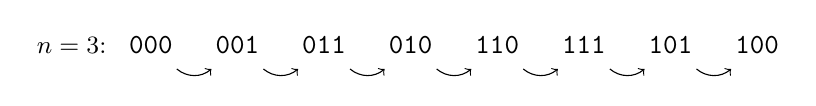
\begin{tikzpicture}[x=1.1cm,y=0.5cm]
\foreach \i/\g in {0/000,1/001,2/011,3/010,4/110,5/111,6/101,7/100}
  \node at (\i,0) {\texttt{\g}};
\foreach \i in {0,...,6} \draw[->] (\i+0.3,-0.6) to[bend right=40] (\i+0.7,-0.6);
\node[left] at (-0.4,0) {\small $n=3$:};
\end{tikzpicture}
\end{center}

\subsection*{Algorithm}
\begin{algorithmic}[1]
\For{$i=0$ \textbf{to} $2^n-1$} print $i\oplus(i\gg1)$ as $n$ bits \EndFor
\end{algorithmic}

\dryrun{$n=2$: $0,1,3,2\to$ \texttt{00, 01, 11, 10}. \checkmark}

\subsection*{C++17 implementation}
\cppfile{bitwise/03_gray_code.cpp}

\begin{complexitybox}
\textbf{Time:} $O(n\,2^n)$ (output size). \textbf{Space:} $O(n\,2^n)$ for
the buffered output.
\end{complexitybox}

\begin{pitfallbox}
\begin{itemize}
  \item Print with leading zeros, most significant bit first.
  \item $2^{16}$ lines $\times$ 17 characters: build one string and print
        once instead of using \texttt{endl} per line.
\end{itemize}
\end{pitfallbox}

\section{A New Number System}
\label{sec:b-new-number}
\source{ICPC 2010--11 Kanpur Online Round (PYQ)}{Easy}

\problemstatement{A ``1-based'' number is a sequence of blocks of the digit
\texttt{0}. A block \texttt{0} sets a flag to $1$; a block \texttt{00} sets it
to $0$; a block of $n>2$ zeros appends $n-2$ copies of the flag to a binary
number. Each number ends with a token \texttt{\#}; the input ends with
\texttt{\textasciitilde}. Print each binary number in decimal (at most 30
bits).}

\begin{patternbox}
Parsing + building a binary number bit by bit: $v\gets2v+\text{bit}$.
\end{patternbox}

\subsection*{Approach and intuition}

Read whitespace-separated tokens; numbers may span several lines, which token
reading handles automatically. Keep the current value and flag, and apply the
rule for each block length. Appending a bit to the right of $v$ is
$v\gets 2v+\text{bit}$ (a left shift by one).

\subsection*{Algorithm}
\begin{algorithmic}[1]
\For{each token $t$}
  \If{$t=$ \texttt{\textasciitilde}} stop
  \ElsIf{$t=$ \texttt{\#}} print $v$; reset
  \ElsIf{$|t|=1$} $flag\gets1$
  \ElsIf{$|t|=2$} $flag\gets0$
  \Else\ repeat $|t|-2$ times: $v\gets2v+flag$
  \EndIf
\EndFor
\end{algorithmic}

\dryrun{\texttt{0 0000 00 000 0 0000 \#}: flag $1$, append \texttt{11};
flag $0$, append \texttt{0}; flag $1$, append \texttt{11}. Binary
\texttt{11011}$=27$. \checkmark}

\subsection*{C++17 implementation}
\cppfile{bitwise/04_new_number_system.cpp}

\begin{complexitybox}
\textbf{Time:} linear in the input size. \textbf{Space:} $O(1)$.
\end{complexitybox}

\begin{pitfallbox}
\begin{itemize}
  \item The PDF prints ``$n2$'' --- a lost subscript for $n-2$.
  \item Reset both the value and the flag between numbers.
\end{itemize}
\end{pitfallbox}

\section{Bitwise Reversion}
\label{sec:b-reversion}
\problemlink{https://codeforces.com/problemset/problem/2153/B}{Codeforces 2153B}
\source{Codeforces 2153B (Notion: Bitwise, 800)}{Easy}

\problemstatement{Given $x,y,z\le10^9$, do non-negative $a,b,c$ exist with
$a\,\&\,b=x$, $b\,\&\,c=y$, $a\,\&\,c=z$?}

\begin{patternbox}
AND conditions only $\Rightarrow$ decide every bit independently.
\end{patternbox}

\subsection*{Approach and intuition}

Look at one bit. If it is set in two of the targets, e.g.\ in $x=a\,\&\,b$ and
$y=b\,\&\,c$, then $a$, $b$ and $c$ all have it, so $a\,\&\,c$ has it too:
the bit must be set in all three. Every other pattern is achievable:
\begin{itemize}
  \item in none: set the bit nowhere;
  \item in exactly one, say $x$: set it in $a$ and $b$ only;
  \item in all three: set it in $a$, $b$, $c$.
\end{itemize}
So the answer is \texttt{NO} iff some bit is set in exactly two of $x,y,z$:
\[
  (x\,\&\,y\,\&\,\lnot z)\mid(x\,\&\,z\,\&\,\lnot y)\mid(y\,\&\,z\,\&\,\lnot x)\ne0.
\]

\subsection*{Algorithm}
\begin{algorithmic}[1]
\State $t\gets(x\,\&\,y\,\&\,\lnot z)\mid(x\,\&\,z\,\&\,\lnot y)\mid(y\,\&\,z\,\&\,\lnot x)$
\State \Return $t=0$
\end{algorithmic}

\dryrun{$x=4=0100_2$, $y=8=1000_2$, $z=12=1100_2$: bit $2$ is in $x$ and $z$
but not $y$ $\Rightarrow$ NO. $x=3$, $y=2$, $z=6$: bit $1$ in all three, bit $0$
only in $x$, bit $2$ only in $z$ $\Rightarrow$ YES. \checkmark\ (Verified on all
$16^3$ triples against brute force.)}

\subsection*{C++17 implementation}
\cppfile{bitwise/05_bitwise_reversion.cpp}

\begin{complexitybox}
\textbf{Time:} $O(1)$ per test. \textbf{Space:} $O(1)$.
\end{complexitybox}

\begin{pitfallbox}
\begin{itemize}
  \item $\lnot z$ on a signed type sets the high bits too; harmless here
        because it is ANDed with non-negative values.
\end{itemize}
\end{pitfallbox}

\section{Deletion Sort}
\label{sec:b-deletion-sort}
\source{Codeforces 2200B (Notion: Bitwise, 800)}{Easy}

\problemstatement{An array of $n\le10$ positive integers. While it is not
non-decreasing, you must delete one element of your choice. Minimise the
number of elements left when the game ends.}

\begin{patternbox}
The tags say bitmask brute force ($2^{10}$ subsets), but a one-line
invariant solves it: \emph{keep an inversion alive}.
\end{patternbox}

\subsection*{Approach and intuition}

If the array is already sorted, the game ends at once: answer $n$. Otherwise
there is an inversion $a_i>a_j$ with $i<j$. As long as more than two elements
remain, delete an element other than $a_i$ and $a_j$: the inversion survives,
so the array is still unsorted and the game continues. With two elements left
(exactly the inversion), delete one; a single element is sorted. Answer $1$.

\subsection*{Algorithm}
\begin{algorithmic}[1]
\State \Return ($a$ non-decreasing) ? $n$ : $1$
\end{algorithmic}

\dryrun{$[1,4,2,3]$: unsorted, answer $1$. $[6,7]$: sorted, answer $2$.
\checkmark}

\subsection*{C++17 implementation}
\cppfile{bitwise/06_deletion_sort.cpp}

\begin{complexitybox}
\textbf{Time:} $O(n)$. \textbf{Space:} $O(n)$.
\end{complexitybox}

\begin{pitfallbox}
\begin{itemize}
  \item Equal neighbours are allowed (``non-decreasing'').
  \item If you do write the bitmask brute force, remember the game stops as
        soon as the array is sorted --- you cannot keep deleting.
\end{itemize}
\end{pitfallbox}

\section{ORXOR}
\label{sec:b-orxor}
\source{AtCoder ABC197 C (Notion: Bitwise)}{Easy--Medium}

\problemstatement{Split an array of $N\le20$ numbers ($<2^{30}$) into
contiguous non-empty blocks; take the OR of each block and the XOR of those
ORs. Minimise the result.}

\begin{patternbox}
$N\le20$ and a ``cut or not'' decision between neighbours $\Rightarrow$
enumerate the $2^{N-1}$ cut masks.
\end{patternbox}

\subsection*{Approach and intuition}

There are $N-1$ gaps; each is cut or not, so a bitmask of $N-1$ bits
describes a partition. For each mask sweep the array, OR-ing into the current
block and closing the block at a cut (or at the end) by xoring its OR into the
total. $2^{19}\cdot20\approx10^7$ steps.

\subsection*{Algorithm}
\begin{algorithmic}[1]
\For{$mask=0$ \textbf{to} $2^{N-1}-1$}
  \State $x\gets0$, $o\gets0$
  \For{$i=0$ \textbf{to} $N-1$}
    \State $o\gets o\mid a_i$
    \If{$i=N-1$ \textbf{or} bit $i$ of $mask$} $x\gets x\oplus o$; $o\gets0$ \EndIf
  \EndFor
  \State $best\gets\min(best,x)$
\EndFor
\end{algorithmic}

\dryrun{$[1,5,7]$: $[1,5][7]$ gives $5\oplus7=2$; $[1][5][7]$ gives $3$;
$[1][5,7]$ gives $1\oplus7=6$; $[1,5,7]$ gives $7$. Minimum $2$. \checkmark}

\subsection*{C++17 implementation}
\cppfile{bitwise/07_orxor.cpp}

\begin{complexitybox}
\textbf{Time:} $O(N\,2^{N-1})$. \textbf{Space:} $O(N)$.
\end{complexitybox}

\begin{pitfallbox}
\begin{itemize}
  \item $N=1$: there is one mask ($0$) and the answer is $a_1$.
  \item Initialise the best with something $\ge2^{30}$, not $0$.
\end{itemize}
\end{pitfallbox}

\section{Jackpot}
\label{sec:b-jackpot}
\source{ICPC 2013--14 Kharagpur Online Round (PYQ)}{Hard}

\problemstatement{A loyalty account starts with $1$ point; once per week the
points either increase by $1$ or double. Alice and Bob each choose a
sub-target, reach it in parallel as fast as possible, and then merge their
points to hit exactly $N$ ($2\le N\le10^9$, $T\le1000$). Find the minimum
number of weeks.}

\begin{patternbox}
Reaching $v$ from $1$ with $+1$/$\times2$ is reading $v$ in binary. Splitting
$N=a+b$ with carries between bits $\Rightarrow$ a \textbf{digit DP over the
bits}.
\end{patternbox}

\subsection*{Approach and intuition}

\textbf{One person.} Work backwards from $v$: if $v$ is even, the last step
could have been a doubling; if odd, it was $+1$. Greedy reversal is optimal,
giving
\[
  f(v)=\bigl(\text{number of bits}-1\bigr)+\bigl(\text{popcount}-1\bigr)=hb(v)+\text{popcount}(v)-1,
\]
where $hb(v)$ is the index of the highest set bit ($f(5)=f(101_2)=2+2-1=3$:
$1\to2\to4\to5$). This formula matches a BFS for all $v<300$.

\textbf{Two people.} They work in parallel, so the answer is
$\min_{a+b=N,\,a,b\ge1}\max(f(a),f(b))$. $N$ is up to $10^9$, so we cannot try
every $a$.

\textbf{Digit DP.} Decide the bits of $a$ and $b$ from the top bit $30$ down
to $0$. At bit $p$ we know which carry $c$ must leave this bit upward; we
choose bits $x,y$ and an incoming carry $c'$ with $x+y+c'=N_p+2c$. The first
set bit of $a$ (from the top) costs $p+1$ (it fixes $hb=p$ and is one set bit);
every later set bit costs $1$. State: (carry $c$, $a$ started?, $b$
started?, cost of $a$ so far) $\mapsto$ minimum cost of $b$. At the end no
carry may enter bit $0$ and both numbers must be non-zero; the answer is
$\min\max(\text{cost}_a,\text{cost}_b)-1$.

\subsection*{Algorithm}
\begin{algorithmic}[1]
\State $dp[c=0][0][0][0]\gets0$, all else $\infty$
\For{$p=30$ \textbf{down to} $0$}
  \For{each state $(c,s_a,s_b,c_a)\mapsto c_b$ and $x,y,c'\in\{0,1\}$ with $x+y+c'=N_p+2c$}
    \State $c_a'\gets c_a+[x](s_a?1:p+1)$, $c_b'\gets c_b+[y](s_b?1:p+1)$
    \State relax $nd[c'][s_a\lor x][s_b\lor y][c_a']$ with $c_b'$
  \EndFor
  \State $dp\gets nd$
\EndFor
\State \Return $\min_{c_a}\max(c_a,dp[0][1][1][c_a])-1$
\end{algorithmic}

\dryrun{$N=10$: $a=b=5$, $f(5)=3$, answer $3$. $N=55$: e.g.\ $15+40$ with
$f(15)=3+4-1=6$, $f(40)=5+2-1=6$; no split does better. Answer $6$. $N=2$:
$1+1$, answer $0$. \checkmark\ (DP checked against the brute-force split
for every $N\le3000$.)}

\subsection*{C++17 implementation}
\cppfile{bitwise/08_jackpot.cpp}

\begin{complexitybox}
\textbf{Time:} $31$ bits $\times$ $512$ states $\times$ $8$ choices
$\approx1.3\cdot10^5$ steps per test, $\approx1.3\cdot10^8$ for $T=1000$.
\textbf{Space:} $O(64)$ states per layer.
\end{complexitybox}

\begin{pitfallbox}
\begin{itemize}
  \item Weeks count \emph{in parallel}: it is $\max$, not $+$.
  \item Both sub-targets must be $\ge1$ (everyone starts with one point).
  \item Trying only $a=\lfloor N/2\rfloor$ fails: $55=27+28$ gives
        $\max(7,6)=7$.
\end{itemize}
\end{pitfallbox}

\section{Express the Number}
\label{sec:b-express}
\source{ICPC 2020--21 Amritapuri Preliminary, problem 2 (PYQ)}{Easy--Medium}

\begin{reconbox}
Only the official solution slides survive (CodeDrills is offline). They say:
``we can use only odd powers; an even power can be written as a sum of odd
powers; if the top power $2^k>x$ has $k$ odd subtract it, if $k$ is even
subtract $2^{k-1}$ twice; once $n\le x$ write it as $A[1]$; impossible for odd
$n$ with $x=0$; complexity $O(\log n)$.'' The statement below is the
reconstruction that matches every line of the slides. The greedy was checked
against an exhaustive DP for all $n\le1500$ and nine values of $x$.
\end{reconbox}

\problemstatement{Given $n$ and $x$, write $n=A_1+A_2+\dots+A_m$ where
$0\le A_1\le x$ and every other term is an \emph{odd} power of two
($2,8,32,128,\dots$). Minimise $m$, or print $-1$ if impossible.}

\begin{patternbox}
Representations with a restricted set of powers of two: process the binary
expansion from the top bit, and rewrite forbidden powers with allowed ones
($2^{2j}=2^{2j-1}+2^{2j-1}$).
\end{patternbox}

\subsection*{Approach and intuition}

While $n>x$ we must spend terms. Let $2^k$ be the top bit of $n$.
\begin{itemize}
  \item $k$ odd: subtract $2^k$ (one term). Using smaller odd powers instead
        would need at least two terms for the same amount.
  \item $k$ even: $2^k$ is not allowed; the largest allowed power below $n$ is
        $2^{k-1}$. Subtract it (one term); after that the top bit is at most
        $k-1$ (odd) and the loop continues.
\end{itemize}
When $n\le x$, the rest becomes $A_1$. If $x=0$ and $n$ is odd we can never
finish, since all odd powers of two are even.

\subsection*{Algorithm}
\begin{algorithmic}[1]
\If{$x=0$ \textbf{and} $n$ odd} \Return $-1$ \EndIf
\State $m\gets0$
\While{$n>x$}
  \State $k\gets hb(n)$; $n\gets n-(k\text{ odd}\ ?\ 2^k:2^{k-1})$; $m\gets m+1$
\EndWhile
\State \Return $m+1$
\end{algorithmic}

\dryrun{$n=10$, $x=3$: top bit $8=2^3$ (odd), $n\to2\le3$: $m=1$, answer $2$
($10=2+8$). $n=10$, $x=0$: $10\to2\to0$, answer $3$ ($A_1=0$, $8$, $2$).
$n=7$, $x=0$: odd, $-1$. \checkmark}

\subsection*{C++17 implementation}
\cppfile{bitwise/09_express_the_number.cpp}

\begin{complexitybox}
\textbf{Time:} $O(\log n)$. \textbf{Space:} $O(1)$.
\end{complexitybox}

\begin{pitfallbox}
\begin{itemize}
  \item $2^0=1$ is an \emph{even} power; it is never allowed.
  \item Use \texttt{unsigned long long} and \texttt{1ULL << k} for large $n$.
\end{itemize}
\end{pitfallbox}

\section{Beautiful XOR}
\label{sec:b-beautiful-xor}
\source{Codeforces 2162C (Notion: Bitwise, 1100)}{Medium}

\problemstatement{Given $a,b\le10^9$. One operation picks $0\le x\le a$
(current $a$) and sets $a\gets a\oplus x$. Transform $a$ into $b$ with at most
$100$ operations, or print $-1$.}

\begin{patternbox}
Constructive xor: first find the invariant (the top bit can never rise), then
use a universal intermediate state --- \textbf{all ones} below the top bit.
\end{patternbox}

\subsection*{Approach and intuition}

\textbf{Impossible case.} If $x\le a$ then $x<2^{hb(a)+1}$, so $a\oplus x$ also
stays below $2^{hb(a)+1}$: the top bit never increases. If $hb(b)>hb(a)$ the
answer is $-1$.

\textbf{Construction.} Let $h=hb(a)$ and $\text{ones}=2^{h+1}-1$.
\begin{itemize}
  \item $a=b$: zero operations.
  \item $a\oplus b\le a$: one operation with $x=a\oplus b$.
  \item otherwise two operations: $x_1=a\oplus\text{ones}$ (its top bit $h$ is
        $0$, so $x_1<2^h\le a$) turns $a$ into $\text{ones}$; then
        $x_2=\text{ones}\oplus b\le\text{ones}$ turns it into $b$.
\end{itemize}

\subsection*{Algorithm}
\begin{algorithmic}[1]
\If{$hb(b)>hb(a)$} \Return $-1$ \EndIf
\If{$a=b$} \Return $[\,]$ \EndIf
\If{$a\oplus b\le a$} \Return $[a\oplus b]$ \EndIf
\State \Return $[a\oplus\text{ones},\ \text{ones}\oplus b]$
\end{algorithmic}

\dryrun{$a=9=1001_2$, $b=6=0110_2$: $a\oplus b=15>9$, so two steps:
$x_1=9\oplus15=6\le9$, $a=15$; $x_2=15\oplus6=9\le15$, $a=6$. $a=292$,
$b=929$: $hb(929)=9>8$, $-1$. \checkmark\ (Any valid sequence is accepted;
checked for all $1\le a,b<64$ against BFS reachability.)}

\subsection*{C++17 implementation}
\cppfile{bitwise/10_beautiful_xor.cpp}

\begin{complexitybox}
\textbf{Time:} $O(1)$ per test. \textbf{Space:} $O(1)$.
\end{complexitybox}

\begin{pitfallbox}
\begin{itemize}
  \item The bound is the \emph{current} $a$, which changes after each
        operation.
  \item For $0$ operations print $0$ and an (empty) second line.
\end{itemize}
\end{pitfallbox}

\section{The 67th XOR Problem}
\label{sec:b-67th}
\source{Codeforces 2218E (Notion: Bitwise, 1200)}{Medium}

\problemstatement{Array $a$ of $n$ values ($\sum n\le3105$, $a_i\le10^9$).
Exactly $n-1$ times: choose an element, let $x$ be its current value, xor
\emph{every} element with $x$, and delete the chosen one. Maximise the value
that remains.}

\begin{patternbox}
Simulate a few steps symbolically: repeated ``xor everything with $x$''
\textbf{telescopes}. What looks like a game collapses to ``max xor of a
pair''.
\end{patternbox}

\subsection*{Approach and intuition}

Write the current array as $a_j\oplus S$, where $S$ is the total mask applied
so far ($S=0$ initially). Removing element $i$ uses $x=a_i\oplus S$, so the new
mask is $S\oplus x=S\oplus a_i\oplus S=a_i$: after every operation the mask
equals the \emph{original} value of the element just removed. Hence the
survivor $j$ ends as $a_j\oplus a_i$, where $i$ is the last removed element.
Any ordered pair $(i,j)$ is achievable, so
\[
  \text{answer}=\max_{i\ne j} a_i\oplus a_j .
\]
Use a binary trie: insert numbers one by one and query the best partner from
the top bit down.

\subsection*{Algorithm}
\begin{algorithmic}[1]
\State insert $a_1$ into the trie; $best\gets0$
\For{$i=2$ \textbf{to} $n$} \State $best\gets\max(best,\textsc{Query}(a_i))$; insert $a_i$ \EndFor
\end{algorithmic}

\dryrun{$[1,2,3]$: pairs give $3,2,1$, answer $3$ (remove $3$: $[2,1]$, then
remove $2$: $[3]$). $[67,67]$: $0$. Sample 3: the best pair is $767\oplus267=1012$.
\checkmark\ (Verified by simulating every removal order on random arrays.)}

\subsection*{C++17 implementation}
\cppfile{bitwise/11_the_67th_xor_problem.cpp}

\begin{complexitybox}
\textbf{Time:} $O(30\,n)$. \textbf{Space:} $O(30\,n)$ trie nodes.
\end{complexitybox}

\begin{pitfallbox}
\begin{itemize}
  \item The survivor is xored with the last removed \emph{original} value,
        not with the xor of all removed values.
  \item Here $\sum n\le3105$, so an $O(n^2)$ double loop also passes; the trie
        is the version that scales.
\end{itemize}
\end{pitfallbox}

\section{Maximize XOR, Minimize Operations}
\label{sec:b-maximize-xor}
\source{Codeforces 2260C (Notion: Bitwise, 1300)}{Medium}

\problemstatement{Given $x,y<2^{29}$. One operation decreases $x$ by $1$ and
increases $y$ by $1$ (only if $x>0$). Find the maximum possible $x\oplus y$ and
the minimum number of operations reaching it.}

\begin{patternbox}
An invariant ($x+y=s$) plus the identity $u+v=(u\oplus v)+2(u\,\&\,v)$
$\Rightarrow$ the maximum is $s$, reached exactly when $u$ is a
\textbf{submask} of $s$.
\end{patternbox}

\subsection*{Approach and intuition}

After $k$ operations the pair is $(u,v)=(x-k,y+k)$ with $u+v=s=x+y$. Since
$u\oplus v=s-2(u\,\&\,v)\le s$, the maximum possible value is $s$, and $u=0$
(i.e.\ $k=x$) already achieves it. Equality needs $u\,\&\,v=0$, i.e.\ $u$ and
$v=s-u$ share no bits, i.e.\ $u$ is a submask of $s$. We need $u\le x$ and want
$k=x-u$ minimal, so we want the \textbf{largest submask of $s$ that is $\le x$}.
Build it greedily from the top: take bit $b$ of $s$ whenever the value stays
$\le x$ (a higher bit outweighs all lower bits together).

\subsection*{Algorithm}
\begin{algorithmic}[1]
\State $s\gets x+y$; $u\gets0$
\For{$b=30$ \textbf{down to} $0$}
  \If{bit $b$ of $s$ \textbf{and} $u\mid2^b\le x$} $u\gets u\mid2^b$ \EndIf
\EndFor
\State \Return $(s,\;x-u)$
\end{algorithmic}

\dryrun{$(6,4)$: $s=10=1010_2$. Bit $3$: $8>6$, skip; bit $1$: $2\le6$, take.
$u=2$, answer $10$ with $6-2=4$ operations ($2\oplus8=10$). $(3,1)$: $s=4$,
$u=0$, answer $4\ 3$. \checkmark\ (Checked for all $x,y<64$.)}

\subsection*{C++17 implementation}
\cppfile{bitwise/12_maximize_xor_minimize_operations.cpp}

\begin{complexitybox}
\textbf{Time:} $O(\log s)$ per test. \textbf{Space:} $O(1)$.
\end{complexitybox}

\begin{pitfallbox}
\begin{itemize}
  \item $s$ can be up to $2^{30}$: loop from bit $30$.
  \item ``Largest submask'' greedy must compare the full partial value with
        $x$, not just the single bit.
\end{itemize}
\end{pitfallbox}

\section{Xor Battle}
\label{sec:b-xor-battle}
\problemlink{https://atcoder.jp/contests/agc045/tasks/agc045_a}{AtCoder AGC045 A}
\source{AtCoder AGC045 A (Notion: Bitwise, harder)}{Hard}

\problemstatement{$x=0$. In round $i=1..N$ ($N\le200$) person $S_i$ may
replace $x$ by $x\oplus A_i$ ($A_i\le10^{18}$) or do nothing. Person $0$ wants
$x=0$ at the end, person $1$ wants $x\ne0$. Who wins with optimal play?}

\begin{patternbox}
Games decided at the end $\Rightarrow$ reason \textbf{backwards}. The future
power of person $0$ is exactly the \textbf{xor span} of their later numbers.
\end{patternbox}

\subsection*{Approach and intuition}

Scan rounds from last to first and let $V$ be the span of person $0$'s numbers
in the rounds already scanned (the future). Claim: person $0$ wins from round
$i$ with current value $x$ iff $x\in V$.
\begin{itemize}
  \item Round of person $0$ with $A_i$: they win iff $x\in V$ or
        $x\oplus A_i\in V$, i.e.\ $x\in V+\{0,A_i\}=\operatorname{span}(V\cup\{A_i\})$.
        So add $A_i$ to the basis.
  \item Round of person $1$: they win if $x\notin V$ or $x\oplus A_i\notin V$.
        If $A_i\notin V$, one of $x$ and $x\oplus A_i$ is outside $V$, so person
        $1$ wins no matter what happened before. If $A_i\in V$, their move
        does not matter.
\end{itemize}
So the answer is $1$ iff some person-$1$ number is not representable by
person $0$'s \emph{later} numbers.

\subsection*{Algorithm}
\begin{algorithmic}[1]
\State basis $\gets\emptyset$
\For{$i=N$ \textbf{down to} $1$}
  \If{$S_i=0$} insert $A_i$
  \ElsIf{$A_i\notin\operatorname{span}(\text{basis})$} \Return $1$
  \EndIf
\EndFor
\State \Return $0$
\end{algorithmic}

\dryrun{$A=(1,2)$, $S=\texttt{10}$: basis $\{2\}$; person~1's $1\notin
\operatorname{span}\{2\}$, answer $1$. $A=(1,1)$: $1\in\operatorname{span}\{1\}$,
answer $0$. \checkmark\ (Checked against a full minimax on random games.)}

\subsection*{C++17 implementation}
\cppfile{bitwise/13_xor_battle.cpp}

\begin{complexitybox}
\textbf{Time:} $O(N\log A)$ per test. \textbf{Space:} $O(\log A)$.
\end{complexitybox}

\begin{pitfallbox}
\begin{itemize}
  \item Only person $0$'s \emph{later} numbers help; earlier ones are already
        spent.
  \item $A_i\le10^{18}<2^{60}$: the basis needs bits $0..59$ (we keep 61).
\end{itemize}
\end{pitfallbox}

\section{XOR Matching}
\label{sec:b-xor-matching}
\problemlink{https://atcoder.jp/contests/abc126/tasks/abc126_f}{AtCoder ABC126 F}
\source{AtCoder ABC126 F (Notion: Bitwise, stretch goal)}{Hard}

\problemstatement{Build a sequence of length $2^{M+1}$ ($M\le17$) in which each
of $0..2^M-1$ appears exactly twice and, for every value, the xor of the
segment between (and including) its two copies equals $K$. Print $-1$ if
impossible.}

\begin{patternbox}
Constructive xor with a symmetric (palindromic) layout; the key fact is
$0\oplus1\oplus\dots\oplus(2^M-1)=0$ for $M\ge2$.
\end{patternbox}

\subsection*{Approach and intuition}

\textbf{Impossible:} $K\ge2^M$ (no segment can have a bit that no element has);
$M=1$, $K=1$ (only $0\,0\,1\,1$-type sequences exist and they give $0$).
\textbf{Small cases:} $M=0$: \texttt{0 0} iff $K=0$; $M=1$, $K=0$:
\texttt{0 0 1 1}.

\textbf{$M\ge2$, $K<2^M$:} print
\[
  \underbrace{0,1,\dots,2^M-1}_{\text{without }K},\;K,\;\underbrace{2^M-1,\dots,1,0}_{\text{without }K},\;K .
\]
\emph{Case $v\ne K$.} The first copy of $v$ is in the ascending half and
the second in the descending half. Between them lie every value $w>v$ (with
$w\ne K$) twice --- once on each side --- and $K$ once. Pairs cancel, the
two copies of $v$ cancel, and the segment xor is $K$.

\emph{Case $v=K$.} The segment is $K$, the whole descending half, $K$. The
descending half is the xor of all values except $K$, which is
$0\oplus K=K$ (the xor of all of $0..2^M-1$ is $0$). With the two copies of
$K$ cancelling, the segment xor is $K$.

\subsection*{Algorithm}
\begin{algorithmic}[1]
\If{$M=0$} \Return $K=0$ ? \texttt{0 0} : $-1$ \EndIf
\If{$M=1$} \Return $K=0$ ? \texttt{0 0 1 1} : $-1$ \EndIf
\If{$K\ge2^M$} \Return $-1$ \EndIf
\State print ascending (skip $K$), $K$, descending (skip $K$), $K$
\end{algorithmic}

\dryrun{$M=2$, $K=1$: \texttt{0 2 3 1 3 2 0 1}. For $3$: segment
$3,1,3$, xor $1$. For $0$: $0,2,3,1,3,2,0$, xor $1$. For $1$:
$1,3,2,0,1$, xor $1$. \checkmark\ (All $M\le4$, $K<40$ checked by a
verifier.)}

\subsection*{C++17 implementation}
\cppfile{bitwise/14_xor_matching.cpp}

\begin{complexitybox}
\textbf{Time:} $O(2^M)$. \textbf{Space:} $O(2^M)$ output.
\end{complexitybox}

\begin{pitfallbox}
\begin{itemize}
  \item $K$ can be up to $10^9$ while $2^M\le131072$: check $K\ge2^M$ first.
  \item $M=1$ is special because $0\oplus1\ne0$.
\end{itemize}
\end{pitfallbox}

